% !TeX root = ./0_article.tex

\documentclass[lettersize,journal]{IEEEtran}
\usepackage{amsmath,amsfonts}
\usepackage{algorithmic}
\usepackage{array}
\usepackage[caption=false,font=normalsize,labelfont=sf,textfont=sf]{subfig}
\usepackage{textcomp}
\usepackage{stfloats}
\usepackage{url}
\usepackage{verbatim}
\usepackage{graphicx}
\usepackage{lipsum}
\hyphenation{op-tical net-works semi-conduc-tor IEEE-Xplore}
\def\BibTeX{{\rm B\kern-.05em{\sc i\kern-.025em b}\kern-.08em
		T\kern-.1667em\lower.7ex\hbox{E}\kern-.125emX}}
\usepackage{balance}

\begin{document}
	\title{IEEE TCAD BBI ARTICLE}
	\author{Geoffrey Chancel}
	\markboth{Journal of \LaTeX\ Class Files,~Vol.~3, No.~4, October~2077}%
	{Shell \MakeLowercase{\textit{et al.}}: A Sample Article Using IEEEtran.cls for IEEE Journals}
	\maketitle
	
	% !TeX spellcheck = en_US
% !TeX root = ./0_article.tex

\begin{abstract}
	This is the abstract.
\end{abstract}

\begin{IEEEkeywords}
	Article submission, IEEE, IEEEtran, journal, \LaTeX, paper, template, typesetting.
\end{IEEEkeywords}
	% !TeX spellcheck = en_US
% !TeX root = ./0_article.tex

\section{Introduction}
%\IEEEPARstart{S}{everal} researches have studied Body Biasing Injection (BBI) in the past few years.
%While this injection method had been \textcolor{orange}{paused/forgotten} for a few years, it has recently regained some interest.
%Among the latest studies, a modeling and simulation flow has been proposed, alongside better platforms allowing to achieve greater reproducibility and a deeper analysis of the mechanisms at works in digital integrated circuits subjected to BBI.
%In addition to that

%	\subsection{Context}
	\IEEEPARstart{N}{owadays}, electronic devices are found in every economic sector, and very often manipulate sensitive and confidential data, such as in bank transactions, Internet of Things (IoT) devices, smartcards, or smartphones.
	To ensure data authenticity and confidentiality, these devices embed cryptographic algorithms.
	While theoretically secure and robust, once implemented on actual devices, these algorithms become fallible by leaking the manipulated data through various physical quantities such as electromagnetic waves, infrared emissions, or sound emissions, not to cite them all, in addition to being sensitive to external disturbances.
	
	In this context, cybersecurity takes place, more specifically hardware security.
	When comes hardware security often comes side-channel attacks and fault injection attacks.
	On the one hand, side-channel attacks take advantage of the circuit leakage by measuring the various physical quantities available.
	On the other hand, fault injection aims at inducing physical disturbances into circuits, with methods like Electromagnetic Fault Injection (EMFI) \cite{mathieuEMFIFirst, mathieuEMFI}, Laser Fault Injection (LFI) \cite{lfiFaultModel}, or Body Biasing Injection (BBI) \cite{bbiOrigin}, not to cite them all.
	Among these methods, EMFI and LFI are widely studied and understood.
	However, despite a resurgence in the past few years, BBI knowledge is still less mature compared to the previously cited methods.
	Therefore, this article is dedicated in presenting our work on Body Biasing Injection.
	
%	\IEEEPARstart{W}{hen} working with cybersecurity, more specifically with hardware security, involving various integrated circuits ranging from smartcards, smartphones, or microcontrollers, various fault injection methods are often considered.
%	We can point out some of the most documented methods such as Electromagnetic Fault Injection (EMFI) \cite{mathieuEMFIFirst, mathieuEMFI}, Laser Fault Injection (LFI) \cite{lfiFaultModel}, or Body Biasing Injection (BBI) \cite{bbiOrigin}, not to cite them all.
%	Our work is dedicated in studying Body Biasing Injection.



	\subsection{Fault injection objectives}
		Before going further in the discussion about BBI, let us first outline the main objectives of fault injection methods.
		Most commonly, they are set up to perform various malicious manipulation on integrated circuits, such as:
		\begin{itemize}
			\item Denial of service (DoS) \textrightarrow\ Stop circuit operation and the related services;
			\item Verification bypass \textrightarrow\ Modify data on the fly to fake authenticity (e.g. to bypass bootloader security);
			\item Confidential data extraction \textrightarrow\ Modify data to perform differential fault analysis.
		\end{itemize}
		To perform these objectives, we can use various injection methods, such as EMFI, LFI or BBI.
		Before presenting our work on BBI further, let us analyze the available and existing BBI platforms in the state-of-the-art.
%		\textcolor{red}{To finish.}

	\subsection{BBI in the state-of-the-art}
	\textcolor{red}{Fait-on vraiment un paragraphe sur les plateformes industrielles comme dans la thèse ?}
		When compared to EMFI, BBI has a smaller state-of-the-art, whether in the amount of scientific papers published or in the amount of industrial platforms proposed.
		Currently, there are ten main works lingering on BBI \cite{bbiOrigin, bbiSecond, bbiThird, bbiColin,japbbi, japbbi2, mybbiCosade, mybbiFdtc2022, mybbifdtc2023, colinFdtc2023}.
		Each one of them made a unique contribution for a better understanding of BBI.

		The first one \cite{bbiOrigin} introduced the technique and presented a Bellcore attack on the targeted IC.
		Then, one year later, another work \cite{bbiSecond} further studied the method, followed by a third work three years later \cite{bbiThird}, introducing an advanced test bench to work and perform attacks with BBI.
		After that, another work presented a low-cost BBI platform, dedicated to WLCSP devices \cite{bbiColin}.

		However, there are still unanswered questions, and the current works aims at bringing more answers thanks to previous and new data.

		Before introducing the present work, let us eventually analyze the industrial platforms proposed by various manufacturers and introduce our own test platform.
		We can distinguish three major actors proposing BBI related products:
		\begin{itemize}
			\item Langer EMV-Technik;
			\item Riscure;
			\item NewAE Technology.
		\end{itemize}

		% !TeX spellcheck = en_US
% !TeX root = ./0_article.tex

\begin{figure}
	\centering
	\subfloat[][Langer]{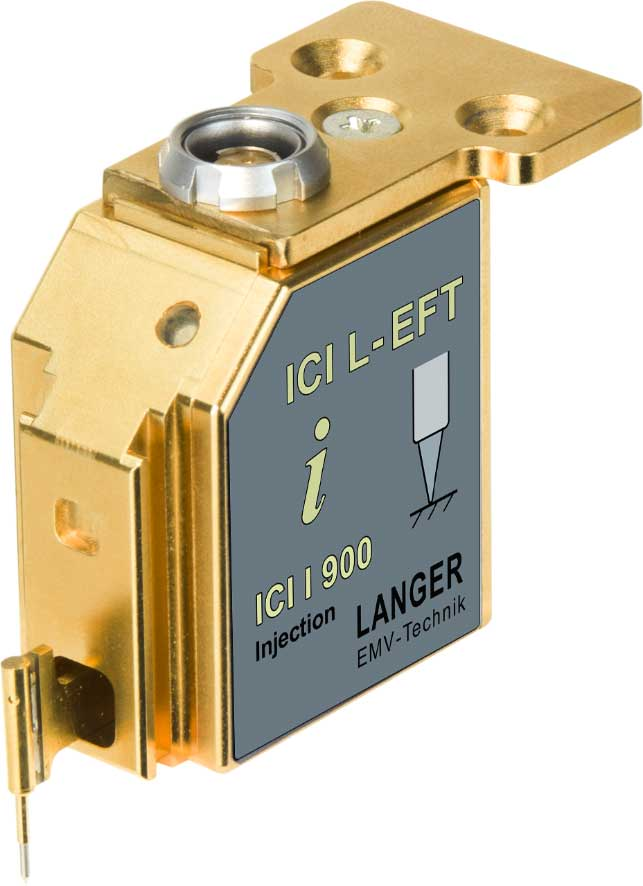
\includegraphics[width=0.2\columnwidth]{./figures/langerBBI.jpg}}
	\hspace{0.1\columnwidth}
	\subfloat[][Riscure]{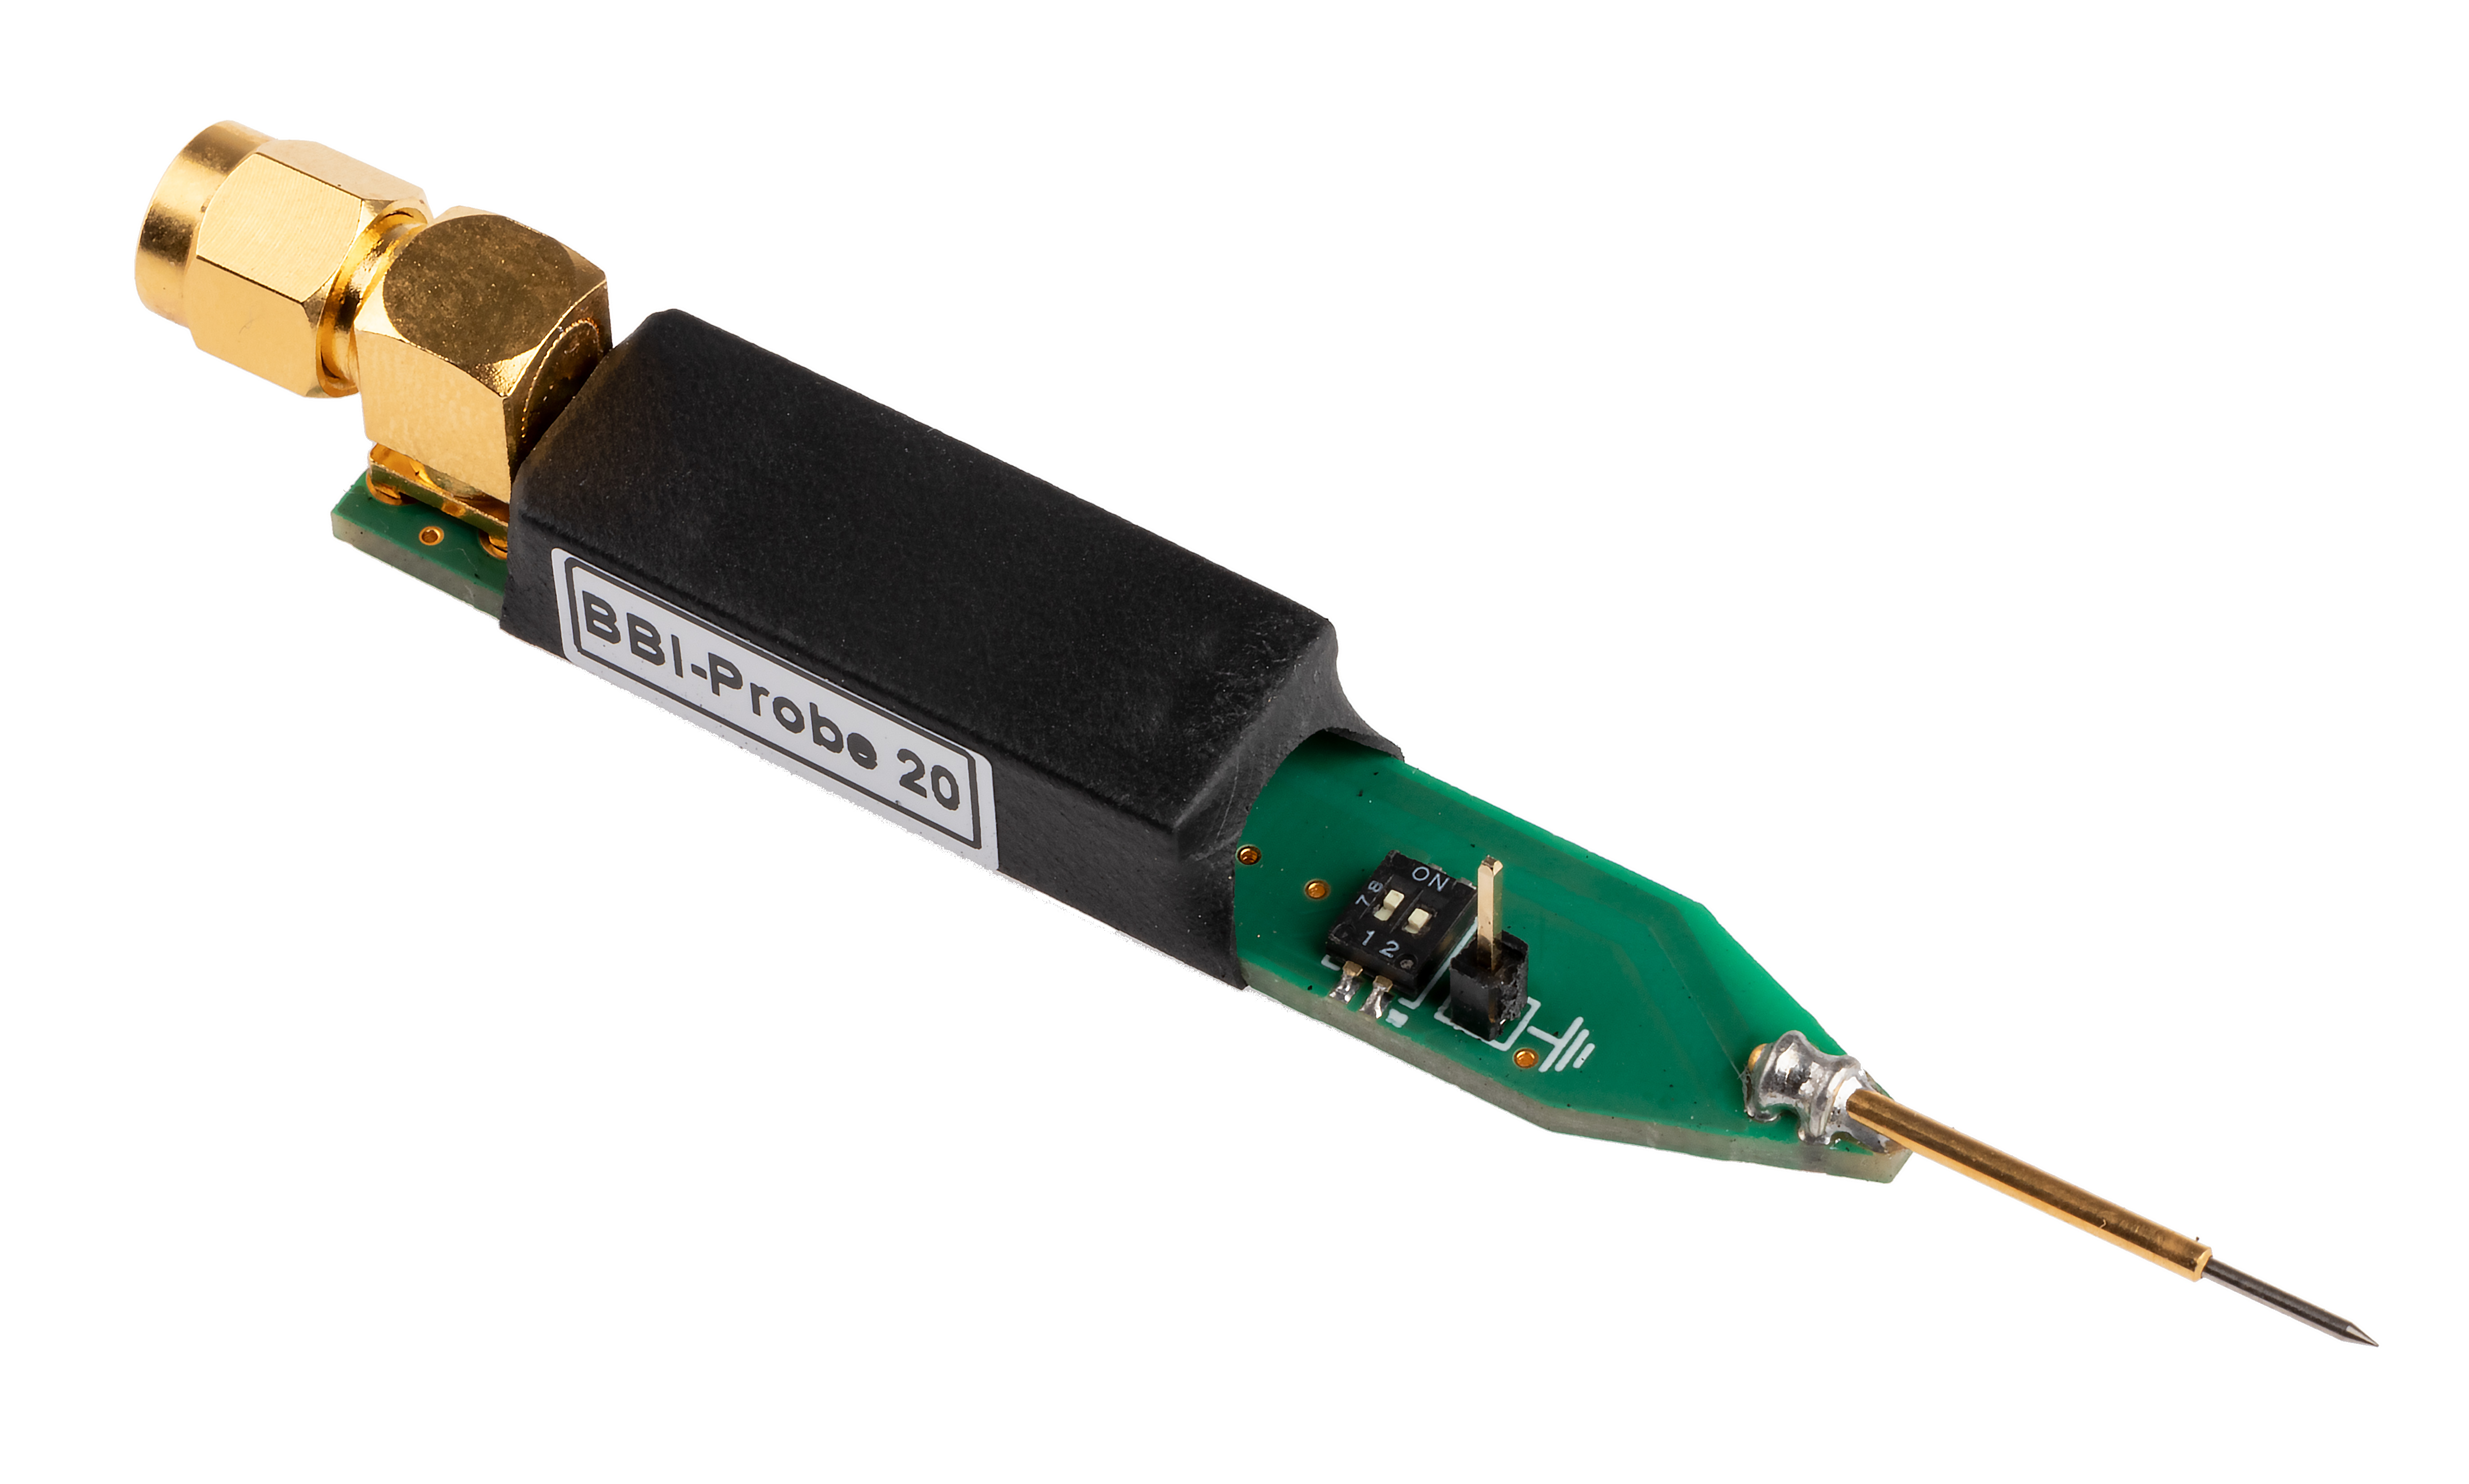
\includegraphics[width=0.425\columnwidth]{./figures/em-fi-bbi-probe-20-black.jpg}}
	\caption{Langer and Riscure BBI probes.}
	\label{riscure_langer}
\end{figure}
		\subsubsection{Langer EMV-Technik platform}
			The German society Langer EMV-Technik proposes an all-in-one and ready-to-use BBI platform composed of two hardware tools:
			\begin{itemize}
				\item A current pulse generator with a metal needle, shown in left in Fig. \ref{riscure_langer};
				\item A general controller called "Burst Power Station", combining a power supply, control and monitor tool and a software.
			\end{itemize}

	\subsection{BBI interrogations}
		With all the work in the state-of-the-art in mind, there are still remaining questions unanswered about BBI, such as:
		\begin{itemize}
			\item What is the spatial resolution of BBI?
			\item What is the time resolution of BBI?
			\item Is thinning the substrate useful in any way?
			\item How BBI induced faults occur?
			\item How to properly model BBI?
		\end{itemize}

	
\end{document}